\documentclass[10pt,letterpaper]{article}
\usepackage[utf8]{inputenc}
\usepackage{amsmath}
\usepackage{amsfonts}
\usepackage{amssymb}
\usepackage{graphicx}
\usepackage{enumerate}
\usepackage{verbatim}
\usepackage{subfig}
\usepackage{gensymb}
\graphicspath{ {ReportImages/} }
\providecommand{\e}[1]{\ensuremath{\times 10^{#1}}}
\usepackage[left=2cm,right=2cm,top=2cm,bottom=2cm]{geometry}
\author{Michael Smith, Haisin Yip, Yang Zhou}
\title{ECSE 415 Project Report}
\begin{document}
\maketitle

\textbf{Part 1}
\paragraph{}
Figs. \ref{training1}, \ref{training2} and \ref{training3} are examples of all the possible poses for a given subject.  These include yaw rotations from -45\degree,-30\degree,0\degree,30\degree and 45\degree at 3 different scales: close, medium and far.  The images were taken on a white background.

Figs. \ref{testing1}, \ref{testing2} and \ref{testing3} show the different testing poses for a given subject.  These include all of the rotations of the training images with the subject facing upwards followed by facing downwards.  In addition, different images were taken of each subject without their glasses, with different facial expressions and with a hat on.

\vspace{5mm}
\textbf{Part 2}
\paragraph{}



\begin{figure}[p]
\subfloat[]{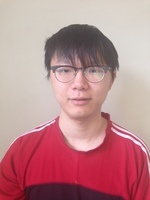
\includegraphics[width = 0.2\textwidth]{Training/gavin_close_0_133_122_32_19.jpg}}
\subfloat[]{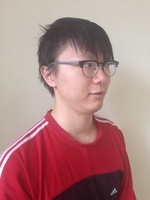
\includegraphics[width = 0.2\textwidth]{Training/gavin_close_30_30_15_124_121.jpg}}
\subfloat[]{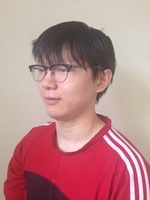
\includegraphics[width = 0.2\textwidth]{Training/gavin_close_-30_126_21_20_124.jpg}}
\subfloat[]{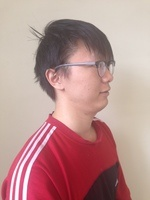
\includegraphics[width = 0.2\textwidth]{Training/gavin_close_45_24_18_118_120.jpg}}
\subfloat[]{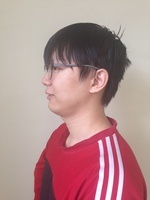
\includegraphics[width = 0.2\textwidth]{Training/gavin_close_-45_31_22_130_122.jpg}}
\caption{Training images at the close, medium and far scales.}
\label{training1}
\end{figure}

\begin{figure}[p]
\subfloat[]{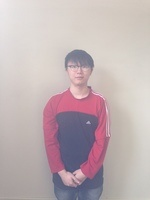
\includegraphics[width = 0.2\textwidth]{Training/gavin_medium_0_57_46_101_90.jpg}}
\subfloat[]{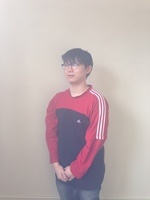
\includegraphics[width = 0.2\textwidth]{Training/gavin_medium_-30_54_47_97_88.jpg}}
\subfloat[]{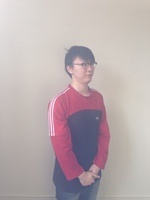
\includegraphics[width = 0.2\textwidth]{Training/gavin_medium_30_106_44_58_84.jpg}}
\subfloat[]{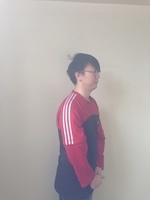
\includegraphics[width = 0.2\textwidth]{Training/gavin_medium_45_58_50_107_93.jpg}}
\subfloat[]{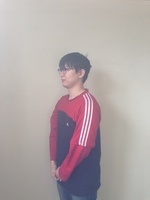
\includegraphics[width = 0.2\textwidth]{Training/gavin_medium_-45_96_50_51_90.jpg}}
\caption{Training images at the medium scale.}
\label{training2}
\end{figure}

\begin{figure}[p]
\subfloat[]{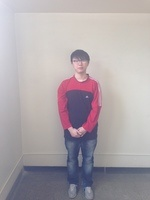
\includegraphics[width = 0.2\textwidth]{Training/gavin_far_0_98_48_63_74.jpg}}
\subfloat[]{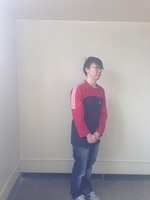
\includegraphics[width = 0.2\textwidth]{Training/gavin_far_30_75_54_109_85.jpg}}
\subfloat[]{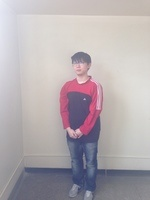
\includegraphics[width = 0.2\textwidth]{Training/gavin_far_-30_96_50_66_78.jpg}}
\subfloat[]{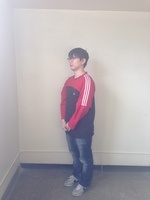
\includegraphics[width = 0.2\textwidth]{Training/gavin_far_-45_60_46_93_75.jpg}}
\subfloat[]{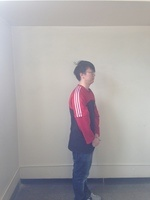
\includegraphics[width = 0.2\textwidth]{Training/gavin_far_45_104_60_68_88.jpg}}
\caption{Training images at the far scale.}
\label{training3}
\end{figure}

\begin{figure}[p]
\subfloat[]{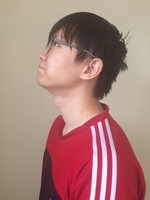
\includegraphics[width = 0.2\textwidth]{Testing/gavin_close_-45_up_134_13_31_118.jpg}}
\subfloat[]{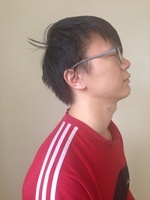
\includegraphics[width = 0.2\textwidth]{Testing/gavin_close_45_up_31_21_144_124.jpg}}
\subfloat[]{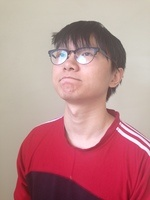
\includegraphics[width = 0.2\textwidth]{Testing/gavin_close_-30_up_37_22_130_118.jpg}}
\subfloat[]{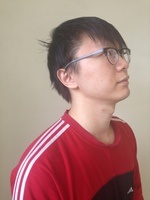
\includegraphics[width = 0.2\textwidth]{Testing/gavin_close_30_up_34_19_143_119.jpg}}
\subfloat[]{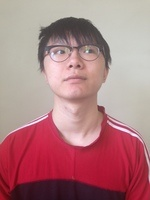
\includegraphics[width = 0.2\textwidth]{Testing/gavin_close_0_up_30_19_122_120.jpg}}
\caption{Testing images of the subject with their head facing upwards.}
\label{testing1}
\end{figure}

\begin{figure}[p]
\subfloat[]{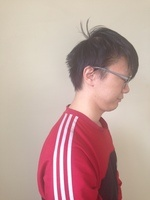
\includegraphics[width = 0.2\textwidth]{Testing/gavin_close_45_down_58_33_139_120.jpg}}
\subfloat[]{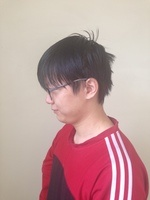
\includegraphics[width = 0.2\textwidth]{Testing/gavin_close_-45_down_25_44_128_129.jpg}}
\subfloat[]{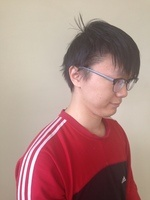
\includegraphics[width = 0.2\textwidth]{Testing/gavin_close_30_down_146_22_54_126.jpg}}
\subfloat[]{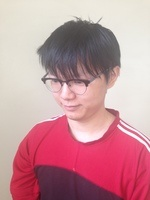
\includegraphics[width = 0.2\textwidth]{Testing/gavin_close_-30_down_29_29_127_120.jpg}}
\subfloat[]{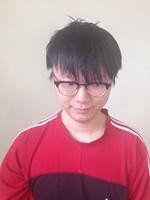
\includegraphics[width = 0.2\textwidth]{Testing/gavin_close_0_down_131_23_41_124.jpg}}
\caption{Testing images of the subject with their head facing downwards.}
\label{testing2}
\end{figure}

\begin{figure}[p]
\subfloat[]{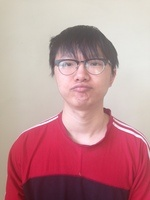
\includegraphics[width = 0.25\textwidth]{Testing/gavin_close_0_smile2_40_25_126_124.jpg}}
\subfloat[]{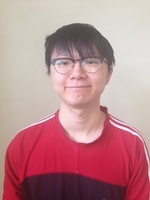
\includegraphics[width = 0.25\textwidth]{Testing/gavin_close_0_smile1_36_26_124_126.jpg}}
\subfloat[]{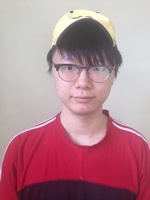
\includegraphics[width = 0.25\textwidth]{Testing/gavin_close_0_hat_38_14_127_128.jpg}}
\subfloat[]{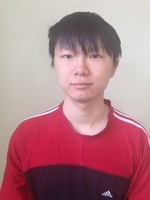
\includegraphics[width = 0.25\textwidth]{Testing/gavin_close_0_glasses_128_16_42_119.jpg}}
\caption{Testing images of the subject with accessories and different facial expressions.}
\label{testing3}
\end{figure}

\end{document}